\section{Paired Accuracy and Length on Fixed Easy Sets}
\label{app:paired-preservation}

\paragraph{Evaluation on identical queries.}
We freeze query IDs using RL anchors $b\in\{100,500,1000\}$ and
$\tau=1$: every selected query has 32/32 correct anchor rollouts.


\begin{figure}[!htbp]
  \centering
  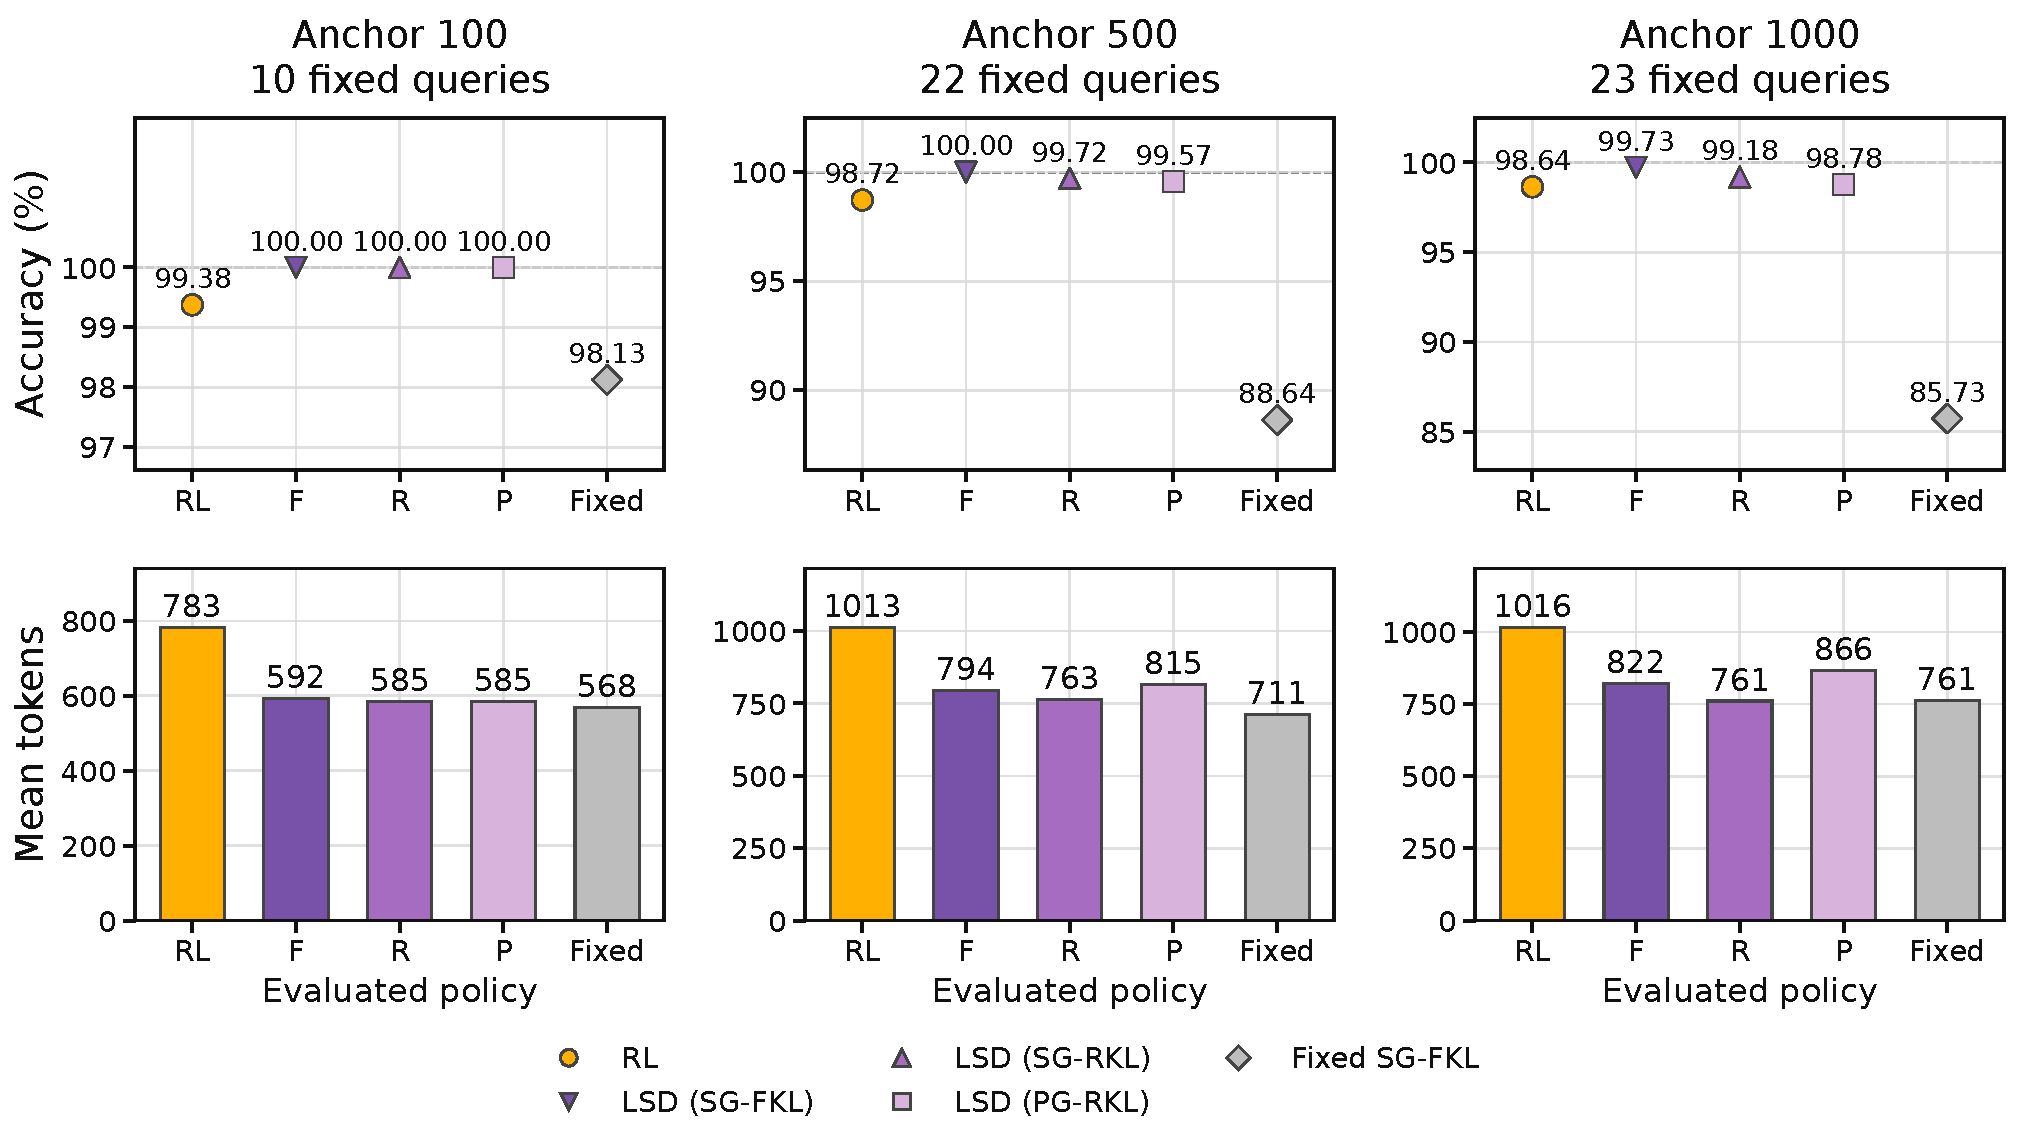
\includegraphics[width=0.84\linewidth]{figures/paired_easy_preservation.pdf}
  \caption{\textbf{Accuracy and length evaluated on the same fixed queries.}
  Each column uses one RL-frozen cohort with $\tau=1$.
  The top row reports empirical accuracy; the bottom row reports mean
  response length. The dashed line marks the 100\% anchor accuracy.
  F, R, and P denote SG-FKL, SG-RKL, and PG-RKL, respectively.
  Every method is evaluated on the
  identical query IDs within a column.}
  \label{fig:paired-preservation}
\end{figure}

\begin{table}[!htbp]
\centering
\small
\caption{\textbf{Paired evaluation on RL-frozen easy sets ($\tau=1$).} $\Delta A$ is the accuracy difference from RL (pp). For $b=1000$, the shared reference is RL step \sharedLSTReferenceStep{}: \sharedLSTReferenceLength{} tokens at 100\% accuracy, the minimum over 345 RL checkpoints.}
\label{tab:paired-preservation}
\resizebox{\linewidth}{!}{%
\begin{tabular}{llrrrr}
\toprule
Anchor & Method & Correct / total & Acc. (\%) & Mean tokens & $\Delta A$ (pp) \\
\midrule
\multirow{5}{*}{$b=100$} & \methodname{RL}{RL} & 318/320 & 99.38 & 783.1 & +0.00 \\
 & \methodname{SGFKL}{LSD (SG-FKL)} & 320/320 & 100.00 & 592.0 & +0.63 \\
 & \methodname{SGRKL}{LSD (SG-RKL)} & 320/320 & 100.00 & 585.3 & +0.63 \\
 & \methodname{PGRKL}{LSD (PG-RKL)} & 320/320 & 100.00 & 585.1 & +0.63 \\
 & \methodname{Fixed}{Fixed SG-FKL} & 314/320 & 98.13 & 568.1 & -1.25 \\
\midrule
\multirow{5}{*}{$b=500$} & \methodname{RL}{RL} & 695/704 & 98.72 & 1013.5 & +0.00 \\
 & \methodname{SGFKL}{LSD (SG-FKL)} & 704/704 & 100.00 & 794.0 & +1.28 \\
 & \methodname{SGRKL}{LSD (SG-RKL)} & 702/704 & 99.72 & 763.0 & +0.99 \\
 & \methodname{PGRKL}{LSD (PG-RKL)} & 701/704 & 99.57 & 815.1 & +0.85 \\
 & \methodname{Fixed}{Fixed SG-FKL} & 624/704 & 88.64 & 710.8 & -10.09 \\
\midrule
\multirow{5}{*}{$b=1000$} & \methodname{RL}{RL} & 726/736 & 98.64 & 1016.2 & +0.00 \\
 & \methodname{SGFKL}{LSD (SG-FKL)} & 734/736 & 99.73 & 822.0 & +1.09 \\
 & \methodname{SGRKL}{LSD (SG-RKL)} & 730/736 & 99.18 & 760.5 & +0.54 \\
 & \methodname{PGRKL}{LSD (PG-RKL)} & 727/736 & 98.78 & 866.1 & +0.14 \\
 & \methodname{Fixed}{Fixed SG-FKL} & 631/736 & 85.73 & 761.4 & -12.91 \\
\bottomrule
\end{tabular}%
}
\end{table}


All three LSD variants use fewer tokens and have higher reported accuracy
than RL on each cohort; all retain 100\% accuracy at $b=100$.

\subsection{The main-table cohort and individual examples}

Table~\ref{tab:paired-main-easy-set} jointly reports accuracy and length
on the easy-query set used in Table~\ref{tab:lsd-best-each-max}, using its
explicitly relaxed RL step-100 cohort ($\tau=0.9$). SG-RKL and PG-RKL
reach 99.43\% and 99.15\% accuracy on these same queries, compared with
98.15\% for RL, while reducing mean length from 997 to 757 and 802
tokens. Fixed produces still shorter responses but lower accuracy,
illustrating why length and correctness must be reported together.
Their hard-query accuracies are 32.50\% and 33.45\%, respectively,
compared with 32.85\% for RL.
SG-FKL reaches 99.10\% and 34.22\% accuracy on the easy and hard
cohorts, with mean lengths of 859 and 2511 tokens, respectively.

% Random-routing control description.
Random Routing matches SG-FKL's EMA teacher ($H=4$), objective, coefficient, and per-step distillation group count. Groups are selected uniformly at random, with GRPO retained on all groups.


\begin{table}[htbp]
\centering
\small
\caption{\textbf{Paired accuracy and response length.} Easy and hard columns use the RL step-100 cohort ($\tau=0.9$) and its complement; LSD and Random Routing Hard Acc. is derived from overall and easy-set accuracy. $\mathrm{LST}_{1000}$ uses the strict step-1000 cohort and shared reference in Table~\ref{tab:paired-preservation}.}
\label{tab:paired-main-easy-set}
\setlength{\tabcolsep}{4pt}
\resizebox{\linewidth}{!}{%
\begin{tabular}{lrrrrrr}
\toprule
\multirow{2}{*}{Method} & \multirow{2}{*}{\shortstack{Avg.\\Pass@1 (\%)}} & \multicolumn{2}{c}{Easy queries} & \multicolumn{2}{c}{Hard queries} & \multirow{2}{*}{$\mathrm{LST}_{1000}$ (\%)} \\
\cmidrule(lr){3-4}\cmidrule(lr){5-6}
& & Acc. (\%) & Mean tokens & Acc. (\%) & Mean tokens & \\
\midrule
\methodname{RL}{RL} & 42.90 & 98.15 & 996.9 & 32.85 & 2329.3 & 19.03 \\
\methodname{SGFKL}{LSD (SG-FKL)} & 44.20 & 99.10 & 859 & 34.22 & 2511 & -3.72 \\
\methodname{SGRKL}{LSD (SG-RKL)} & 42.80 & 99.43 & 757.2 & 32.50 & 2395.0 & -10.92 \\
\methodname{PGRKL}{LSD (PG-RKL)} & 43.56 & 99.15 & 801.6 & 33.45 & 2392.5 & 1.45 \\
Random Routing & 22.08 & 89.74 & 895.0 & 9.78 & 2006.6 & -11.00 \\
\methodname{Fixed}{Fixed SG-FKL} & 30.44 & 94.89 & 690.6 & 18.72 & 1322.8 & -10.81 \\
\bottomrule
\end{tabular}%
}
\end{table}


\begin{figure}[htbp]
  \centering
  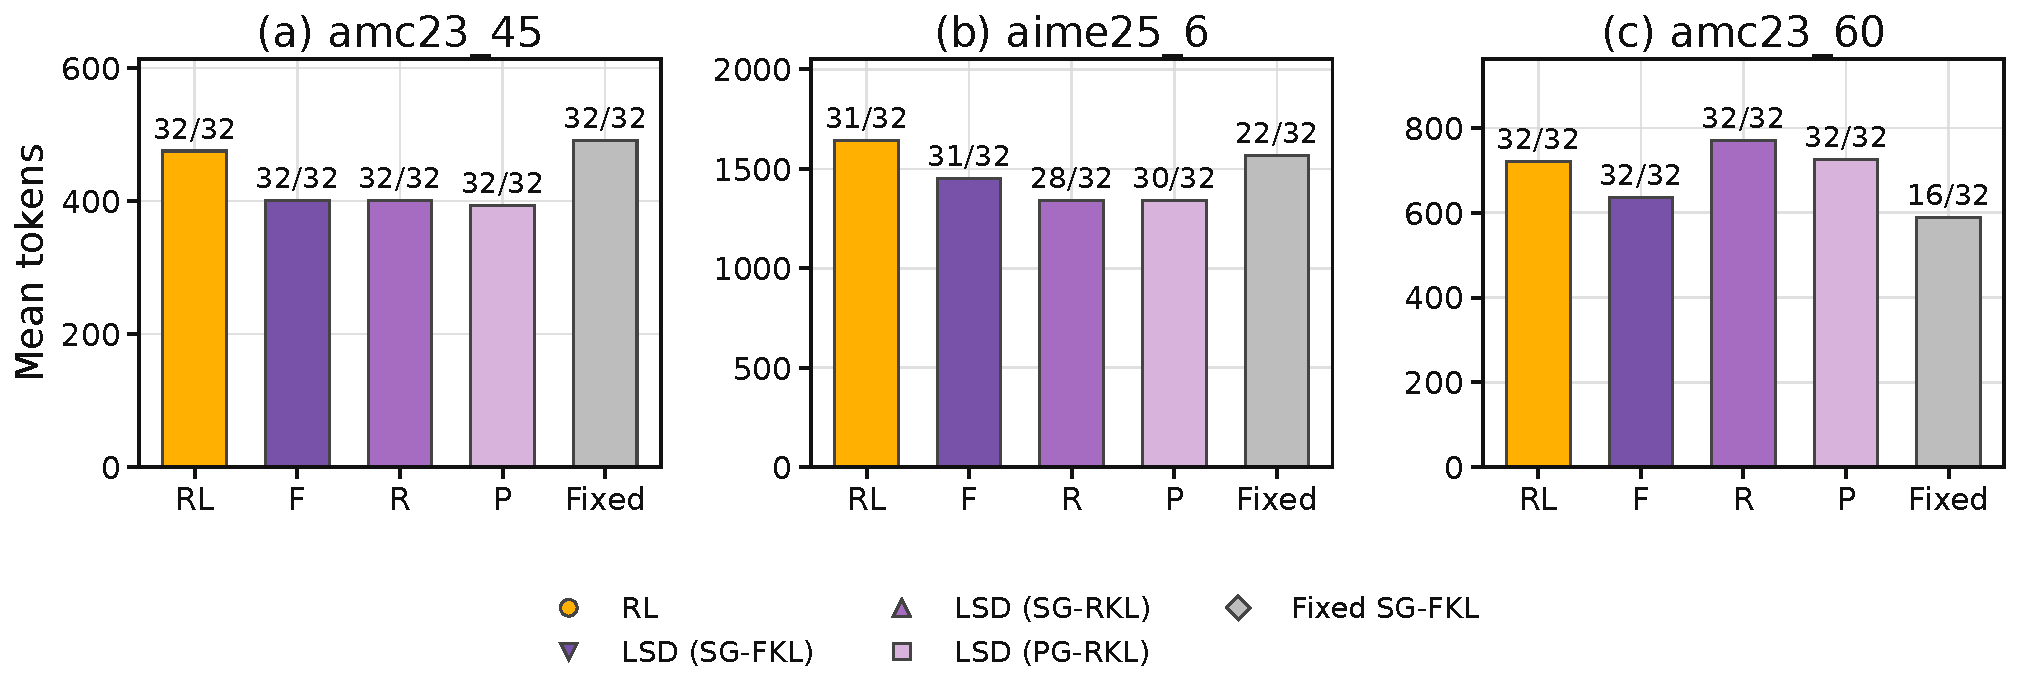
\includegraphics[width=\linewidth]{figures/paired_query_examples.pdf}
  \caption{\textbf{Query-level examples from the strict step-1000 cohort.}
  Bar height is mean response length; labels give correct rollouts out
  of 32. All three queries were answered correctly in all 32 RL anchor
  rollouts. The examples include unchanged correctness, an LSD
  regression, and a Fixed regression. F, R, and P denote SG-FKL,
  SG-RKL, and PG-RKL, respectively.}
  \label{fig:paired-query-examples}
\end{figure}

For \texttt{amc23\_45}, RL and all three LSD variants answer 32/32
correctly, while mean length falls from 475.2 to 401, 400.4, and
393.2 tokens under SG-FKL, SG-RKL, and PG-RKL, respectively.
This is a direct example of shortening at identical observed accuracy.
It is selected near the median joint length reduction among queries
with 32/32 correctness for RL, SG-RKL, and PG-RKL and shorter responses
under both RKL variants.

The other examples expose the limits of the aggregate result.
For \texttt{aime25\_6}, correctness falls from RL's 31/32 to 28/32
under SG-RKL and 30/32 under PG-RKL despite shorter responses;
SG-FKL retains 31/32 while reducing mean length from 1640.9 to 1453 tokens.
For \texttt{amc23\_60}, RL and all three LSD variants retain 32/32
correctness; SG-FKL reduces mean length from 720.4 to 637 tokens, while Fixed drops
to 16/32 while shortening its response.
These examples are selected as the largest respective correctness
regressions among shortened queries in the cohort, so that the case
analysis includes failure cases as well as successful preservation.

